\documentclass[10pt,twocolumn]{article}
\usepackage[margin=1in]{geometry}
\usepackage{times}
\usepackage{graphicx}
\usepackage{amsmath}
\usepackage{hyperref}
\usepackage{tikz}
\usepackage{placeins}
\usetikzlibrary{shapes.geometric, arrows.meta, positioning}
\tikzstyle{process} = [rectangle, rounded corners, minimum width=3cm, minimum height=1cm, text centered, draw=black, fill=gray!10]
\tikzstyle{arrow} = [thick,->,>=stealth]


\title{Cancer Prediction using Logistic Regression}
\author{
    Andrei Sheremet \\
    IT-Universitetet i København \\
    \texttt{andsh@itu.dk}
    \and
    Nam Tran \\
    IT-Universitetet i København \\
    \texttt{hotr@itu.dk}
}

\date{}

\begin{document}
\maketitle

\begin{abstract}
Cancer prediction is a critical area of research in medical diagnostics. In this project, we aim to build a logistic regression model to predict cancer using features extracted from dermoscopic images. We explore various features, including those from image preprocessing and a "hair" feature indicating preprocessing type.
\end{abstract}

\section{Introduction}

Cancer is a major global health concern, with early detection being absolutely crucial to improve human's survival rates. Skin cancer, including melanoma, is particularly treatable if identified early. In dermatology, dermoscopic imaging enables clinicians to visualize skin lesions, and recent advances in data science offer tools to assist diagnosis by identifying malignant features automatically.

This project explores the use of machine learning, specifically logistic regression for predicting skin cancer using features derived from dermatoscopic images. Our project aim to build an interpretable, efficient model that can classify lesions as malignant or benign, supporting diagnostic workflows with transparent, data-focused insights.

\subsection*{Problem Statement}

We frame this as a binary classification task: predicting the presence or absence of cancer from image-derived features. Given that a misclassified lesion can delay treatment, our goal is to minimize such errors while maintaining overall accuracy. Logistic regression is chosen due to its interpretability and strong baseline performance in binary tasks. We will dive deeper on why we choose this specific Machine Learning model later.

\subsection*{Objectives}

The project has three primary goals:
\begin{itemize}
    \item Build a logistic regression model to classify lesions as malignant or benign based on extracted features.
    \item Evaluate model performance using metrics such as accuracy and F1-score.
    \item Compare a baseline model (with three features) to an extended version using a fourth “hair” feature.
\end{itemize}

\subsection*{Methodology Overview}

After extracting and scaling features from each lesion, we split the dataset (80/20 stratified sampling) into training and test sets to preserve class distribution. We train a logistic regression model using scikit-learn with default settings and L2 regularization. For the extended model, we include the hair feature to test its effect on performance.

We evaluate both models using accuracy and F1-score, and compare confusion matrices to understand error types (false positives/negatives). Feature importance is analyzed via model coefficients.

\section{Dataset Description}
The dataset is based on the HAM10000 collection, as described in \href{https://www.sciencedirect.com/science/article/pii/S235234092031115X}{this article}. It contains dermatoscopic images of skin lesions, along with metadata and diagnostic labels. We used a CSV file with pre-extracted features for modeling. For this project, we convert the labels into a binary target: malignant (e.g., melanoma, BCC) vs. benign (e.g., nevus, keratosis). The dataset includes masks for each lesion, aiding in image preprocessing and feature extraction.

We extract four main features:
\begin{itemize}
    \item \textbf{Asymmetry (A)} – Measures shape imbalance, as malignant lesions tend to be more asymmetric.
    \item \textbf{Compactness (B)} – Quantifies border irregularity, common in cancerous lesions.
    \item \textbf{Color Variation (C)} – Captures lesion color diversity using k-means clustering.
    \item \textbf{Hair (H)} – Derived from morphological filtering and inpainting; represents preprocessing artifacts.
\end{itemize}

The baseline model uses A, B, and C; the extended model adds H. Features are normalized to [0, 1] to aid in training.

\section{Model Building}
\subsection{Logistic Regression}

Logistic regression is a supervised machine learning algorithm commonly used for binary classification tasks. It models the probability that a given input belongs to a particular class by applying the logistic (sigmoid) function to a linear combination of input features:

\[
P(y = 1 \mid \mathbf{x}) = \frac{1}{1 + e^{-(\beta_0 + \beta_1 x_1 + \cdots + \beta_n x_n)}}
\]

where \( \mathbf{x} = (x_1, \ldots, x_n) \) is the input feature vector, and \( \beta_i \) are the learned coefficients.

Unlike linear regression, which predicts continuous values, logistic regression produces probabilities in the range \([0, 1]\), making it particularly suitable for tasks such as cancer prediction, where the output is binary (malignant vs. benign).

\subsection{Model Choice Justification}

We chose logistic regression for several reasons:
\begin{itemize}
    \item \textbf{Interpretability:} The coefficients in logistic regression offer information on how each characteristic contributes to the prediction, which is important in medical contexts.
    \item \textbf{Simplicity:} Logistic regression is computationally efficient, easy to implement, and well suited for small to medium-sized data sets.
    \item \textbf{Baseline Comparisons:} It provides a strong baseline model, which makes it easier to evaluate whether more complex models offer substantial performance gains.
\end{itemize}

While more complex models such as decision trees or neural networks can capture non-linear relationships, our primary goal was to establish a clean, interpretable baseline model. Logistic regression strikes a good balance between performance and explainability.

\subsection{Feature Description}
To enable effective classification of skin lesions, we extracted a set of handcrafted features from lesion masks and images. These features were designed to capture shape, texture, and color properties relevant to cancer detection. The main categories are:

\begin{itemize}
    \item \textbf{Asymmetry:} Calculated by rotating and comparing flipped segments of the mask. High asymmetry suggests malignancy.
    
    \item \textbf{Compactness:} Measures how close the shape is to a circle using the formula
    \[
    \text{Compactness} = 1 - \frac{4 \pi \cdot \text{Area}}{\text{Perimeter}^2}
    \]
    Less compact lesions may indicate irregular, cancerous borders.
    
    \item \textbf{Color Variation (Multicolor Rate):} Computed by clustering lesion pixels (using KMeans) and measuring the maximum distance between color cluster centers in RGB space. High variation often correlates with malignancy.
    
    \item \textbf{Hair Feature:} Using morphological filtering and inpainting (OpenCV’s blackhat + inpaint), we computed the proportion of detected hair pixels in each image. This was included as a binary feature to indicate whether hair was present and processed.
\end{itemize}

All features were normalized to the \([0, 1]\) range to ensure compatibility with logistic regression. We trained two model versions — one with the hair-related feature included, and one without — to assess its impact on performance.

The dataset was split into 80\% training and 20\% testing using stratified sampling to preserve class balance.

\begin{figure}[h]
\centering
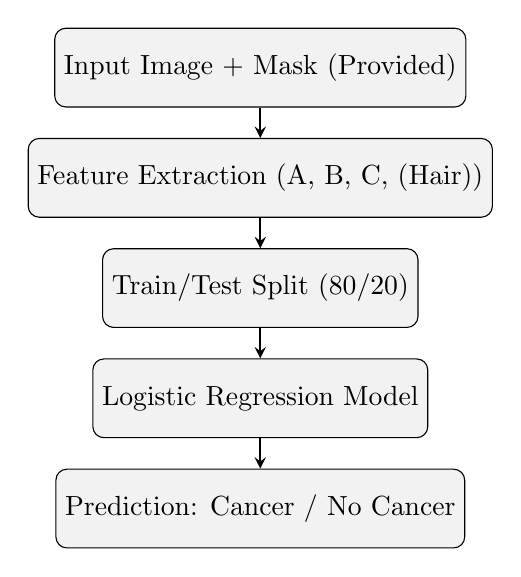
\begin{tikzpicture}[node distance=1.4cm]

\node (input) [process] {Input Image + Mask (Provided)};
\node (features) [process, below of=input] {Feature Extraction (A, B, C, (Hair))};
\node (split) [process, below of=features] {Train/Test Split (80/20)};
\node (model) [process, below of=split] {Logistic Regression Model};
\node (output) [process, below of=model] {Prediction: Cancer / No Cancer};

\draw [arrow] (input) -- (features);
\draw [arrow] (features) -- (split);
\draw [arrow] (split) -- (model);
\draw [arrow] (model) -- (output);

\end{tikzpicture}
\caption{Overview of the model pipeline.}
\label{fig:pipeline}
\end{figure}



\section{Results and Evaluation}
\subsection{Evaluation Metrics}
We evaluated model performance using accuracy, F1 score, and the confusion matrix. Accuracy provides a general sense of correctness, but given the potential class imbalance in our dataset, the F1 score is more informative. Balances both precision and recall, making it a better indicator of how well the model handles both classes.
\subsection{Baseline Model}
The baseline model was trained using three features extracted from each image: Asymmetry (A), Border Compactness (B), and Color Variation (C). We used logistic regression to classify skin lesions as benign or malignant.

On the test set, the model achieved \textbf {an accuracy of 0.587} and \textbf{an F1 score of 0.600}. While the accuracy was modest, the F1 score indicates reasonable performance in handling both false positives and false negatives.

\begin{figure}[h]
    \centering
    \includegraphics[width=0.45\textwidth]{matrix_base.png}
    \caption{Confusion Matrix – ABC Baseline Model}
    \label{fig:matrix_baseline}
\end{figure}

The confusion matrix (Figure~\ref{fig:matrix_baseline}) shows that the model correctly identified 123 malignant cases and 110 benign cases, but misclassified 71 malignant and 93 benign samples.

\subsection{Extended Model}
The extended model added a fourth feature (H), representing the proportion of hair pixels in each image. The same logistic regression algorithm was used for consistency. This model achieved a slightly higher accuracy of 0.602 and an F1 score of 0.609.

\begin{figure}[h]
    \centering
    \includegraphics[width=0.45\textwidth]{matrix_extended.png}
    \caption{Confusion Matrix – ABCH Extended Model}
    \label{fig:matrix_extended}
\end{figure}

Compared to the baseline, the extended model slightly improved correct benign classifications (116 vs. 110) while keeping malignant prediction performance the same (123 true positives). False negatives remained unchanged at 71, but false positives were reduced from 93 to 87. These small improvements suggest that \textbf{ the hair feature (H) contributed useful but limited additional signal.}

\subsection{Insights}
While both models used a simple logistic regression classifier, we observed that even small changes in feature engineering impacted the results. Adding the hair-based feature (H) slightly improved the accuracy and F1 score, suggesting it provides some additional discriminative value.

Interestingly, we also experimented with normalizing all feature values to the \([0, 1]\) range. Contrary to expectations, the performance worsened: accuracy dropped to 0.588 and F1 score to 0.579. This suggests that the logistic regression model may have benefited from the original raw scale of some features, particularly the asymmetry (A) score. 

These observations highlight that even basic modeling decisions—such as whether or not to normalize—can significantly affect outcomes and should be guided by empirical testing rather than assumptions.

\subsection{Open Question: Feature Comparison}
While our extended model showed slight improvements, a deeper analysis of individual feature contributions revealed a more nuanced picture. As shown in Figure~\ref{fig:feature_importance}, features B (border compactness) and C (color variation) provided the highest discriminative power, while the asymmetry feature (A), despite being intuitively useful, contributed less than expected.
\begin{figure}[ht]
\centering
\includegraphics[width=0.42\textwidth]{feature_correlation.png} 
\caption{Feature importance comparison based on logistic regression weights.}
\label{fig:feature_importance}
\end{figure}

This raises an open question: to what extent are our handcrafted features complementary, and could feature correlation or redundancy be limiting model performance? Future work could explore feature selection techniques or employ model interpretation tools such as SHAP or the importance of permutation of permutations to better understand these dynamics.
\subsection{Limitations}

Several limitations affected the model's overall performance. First, the handcrafted features—while intuitive—may not capture the full complexity of lesion characteristics, especially compared to deep learning-based approaches. The asymmetry score, for example, was sensitive to how the lesion was cropped and rotated, potentially introducing noise. Additionally, while the hair detection feature (H) added slight value, its accuracy is uncertain. As shown in Figure~\ref{fig:hair_validation_scatter}, the correlation between our automatic hair score and manual hair labels is weak and noisy, suggesting our detection method may need refinement. Finally, since the dataset already provided masks, we did not assess performance on raw images without preprocessing, which limits real-world applicability.

\begin{figure}[htbp]
\centering
\includegraphics[width=0.45\textwidth]{hair_validation_scatter.png}
\caption{Scatter plot comparing manual hair labels (x-axis) and automatically detected hair ratio (y-axis). Weak correlation suggests limited reliability of the hair detection algorithm.}
\label{fig:hair_validation_scatter}
\end{figure}


\section{Conclusion}
We successfully built a working skin cancer prediction model using logistic regression and handcrafted image features. Despite the model’s simplicity, it achieved reasonable accuracy and F1 scores, with the extended version slightly outperforming the baseline. Our experiments showed that even small changes—such as adding a hair detection feature or normalizing input values—can impact model performance.

Interestingly, normalization and asymmetry normalization did not improve results, highlighting that empirical testing should guide design decisions over assumptions. The strongest predictors were border compactness and color variation, while asymmetry, despite its intuitive appeal, contributed less than expected.

While the model has limitations—including potentially noisy features, reliance on provided masks, and weak correlation in hair detection—this project demonstrates that meaningful predictions can still be extracted using basic tools. Future improvements could involve feature selection, more robust hair analysis, or moving toward deep learning techniques for end-to-end training on raw images.

\end{document}
